\documentclass[a4paper]{ctexart} %CTEX报告文章格式
\usepackage[top=3cm,bottom=2cm,left=2cm,right=2cm]{geometry} % 页边距
\usepackage{amsthm}

\usepackage{graphics} %图片
\usepackage{indentfirst}
\usepackage[hyperref=true,backend=biber,sorting=none,backref=true]{biblatex}
\addbibresource{plant-ref.bib}
\setlength{\parindent}{2em}
\title{深度学习在植物识别中的应用}
\author{王健$^1$}

\begin{document}
	\maketitle
	\begin{center}
		(1 中国科学院软件研究所,北京 100190, yt4766269@126.com)
	\end{center}
\textbf{关键词}:深度学习,计算机视觉,植物,叶片

\textbf{摘要}\quad 本文将图像识别研究的最新进展应用于植物图像识别,使用深度学习算法进行叶片分类研究,探究了三种流行的卷积神经网络模型在植物叶片分类上的效果,在经过25个训练循环之后,三种神经网络模型在北美184种植物叶片数据集上均取得了较好的分类效果。

\section*{引言}
为了保护物种多样性,了解一个地区的植物物种组成是非常重要的。但是传统的植物物种判别手段不仅非常复杂和耗时,而且要求识别人掌握全面的植物知识。而如今,物种自动识别方向的研究正引起人们的兴趣。我们可以通过照相机、手机等设备进行图像采集,然后调用物种判别算法,对采集到的图像数据进行分析,最终得到具体物种信息。而在上述流程中,物种判别算法的准确率影响着物种自动识别的好坏,因此物种判别算法起着至关重要的作用。

而随着深度学习理论的发展与计算机视觉技术的进步,近年来涌现出了一大批优秀的深度学习模型,其中包括Vgg\parencite{vgg},Resnet\parencite{resnet},Densenet\parencite{densenet}等,这些深度学习模型在Imagenet\parencite{imagenet}的1000种图像分类的数据集上取得了很好的结果。而植物图像分类问题与Imagenet图像分类问题类似,均可以用深度学习模型很好的解决。因此,本文将如上三种深度学习模型应用于植物图像识别,进行植物叶片照片的分类研究。

\section*{深度学习与图像识别}
2006年,Hinton提出了深度学习。之后深度学习在诸多领域取得了巨大成功,受到广泛关注。神经网络能够重新焕发青春的原因有几个方面:首先,大规模训练数据的出现在很大程度上缓解了训练过拟合的问题。例如,ImageNet训练集拥有上百万个有标注的图像。其次,计算机硬件的飞速发展为其提供了强大的计算能力,一个GPU芯片可以集成上千个核。这使得训练大规模神经网络成为可能。第三,神经网络的模型设计和训练方法都取得了长足的进步。

而深度学习在物体识别中有非常重要的应用,其中最重要的进展体现在ImageNet ILSVRC挑战中的图像分类任务。传统计算机视觉方法在此测试集上最低的错误率是26.172\%。2012年,Hinton的研究小组利用卷积网络把错误率降到了15.315\%。在此之后,不断有新的网络结构被提出出来,网络的深度也不断增加,2014年,Andrew Zisserman等人提出了VGG全卷积网络,在Imagenet数据集上取得了6.8\%的top-5错误率。2015年,微软亚洲研究院的何凯明等人提出了Resnet,将网络层数增加到152层,在Imagenet数据集上取得了3.57\%的top-5错误率。2016年,康奈尔大学的Kilian Q. Weinberger等人,开发出Densenet网络结构,取得了5.3\%的top-5错误率,同时大大加快的网络训练的速度。

虽然深度学习在ImageNet上取得了巨大成功,但是很多应用的训练集是较小的,在此种情况下,可以将ImageNet上训练得到的模型作为起点,利用目标训练集和反向传播对其进行继续训练,将模型适应到特定的应用。此时ImageNet起到预训练的作用。

本文使用了以上三种优秀的神经网络结构,采用了Leafsnap数据集,利用植物的叶片照片进行植物图像分类的研究。

\section*{实验部分}
\subsection*{数据集}
本文使用了Leafsnap\parencite{leafsnap}数据集,数据集中包括美国北部184种植物叶子图片,共计23,147张图片,其中部分图片如图1所示例。这些数据图片在光照,阴影,清晰度等方面变化很大。该数据集可以通过如下网站下载得到:http://leafsnap.com/dataset/
\begin{figure*}[htbp]
	\centering
	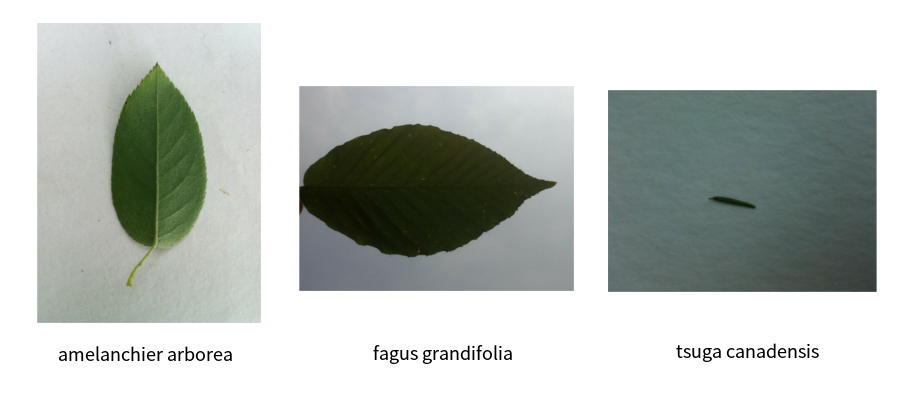
\includegraphics[width=0.75\textwidth]{img1.png}
	\caption{数据集原图}
	\label{figure}
\end{figure*}


在获得数据集之后,需要对原始图片进行预处理,首先将所有图片按照3:1的比例生成训练集与测试集,对于所有图片,将其从图像中间裁剪至256像素×256像素大小,然后进一步随机裁剪至224×224像素大小,然后将图像随机水平翻转,最后将图像归一化,归一化后的图片如图2所示。

\begin{figure*}[htbp]
	\centering
	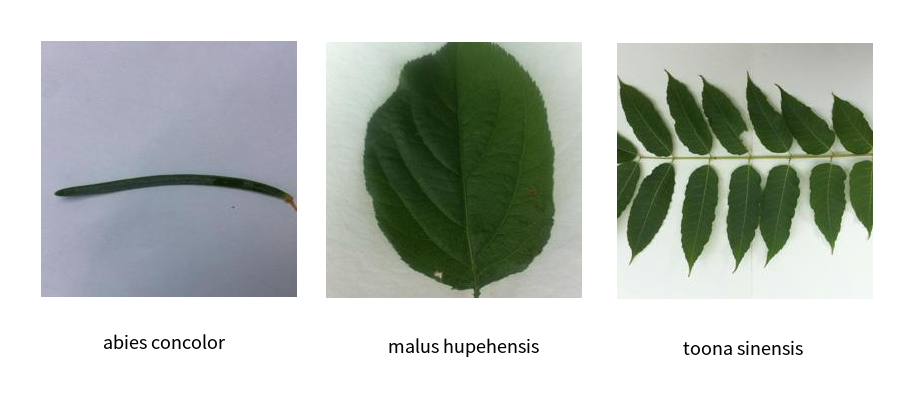
\includegraphics[width=0.75\textwidth]{img2.png}
	\caption{预处理后图片}
	\label{figure}
\end{figure*}

\subsection*{训练步骤}
在数据预处理完成和选定模型完成之后,可以进行训练参数的设定,这里,我们将三种模型的参数统一设定如下:
\begin{itemize}
	\item 学习速率:0.001
	\item 动量:0.9
	\item batch\_size:4
\end{itemize}
同时,在训练过程中采用了已经预先在Imagenet数据集上训练好的网络参数数据作为预训练的结果。

\subsection*{训练结果}
vgg19在该数据集上获得了92.54\%的准确率,训练的loss曲线如图3所示:

\begin{figure*}[htbp]
	\centering
	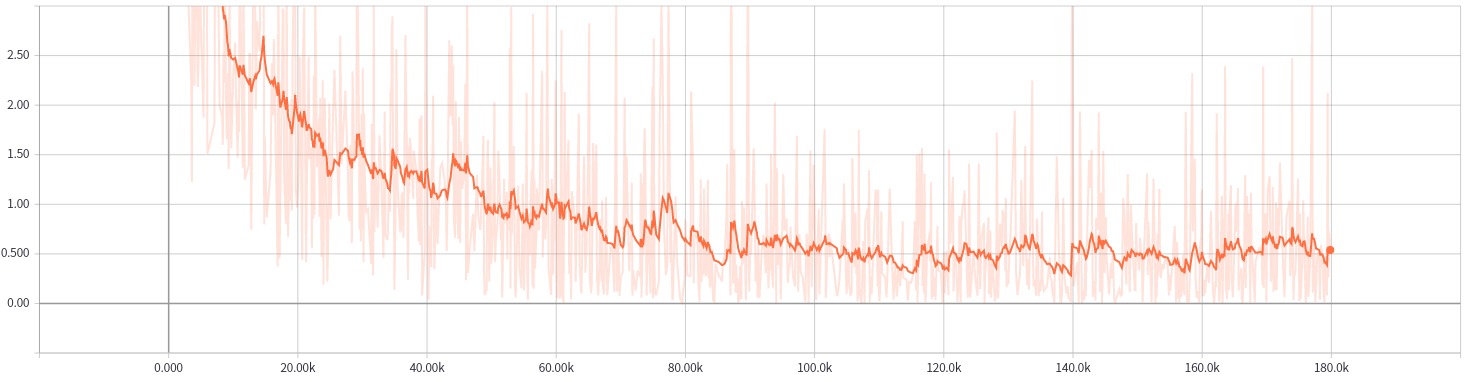
\includegraphics[width=0.75\textwidth]{vgg.png}
	\caption{vgg训练曲线}
	\label{figure}
\end{figure*}

Resnet在该数据集上获得了93.25\%的准确率,训练时的loss曲线如图4所示:

\begin{figure*}[htbp]
	\centering
	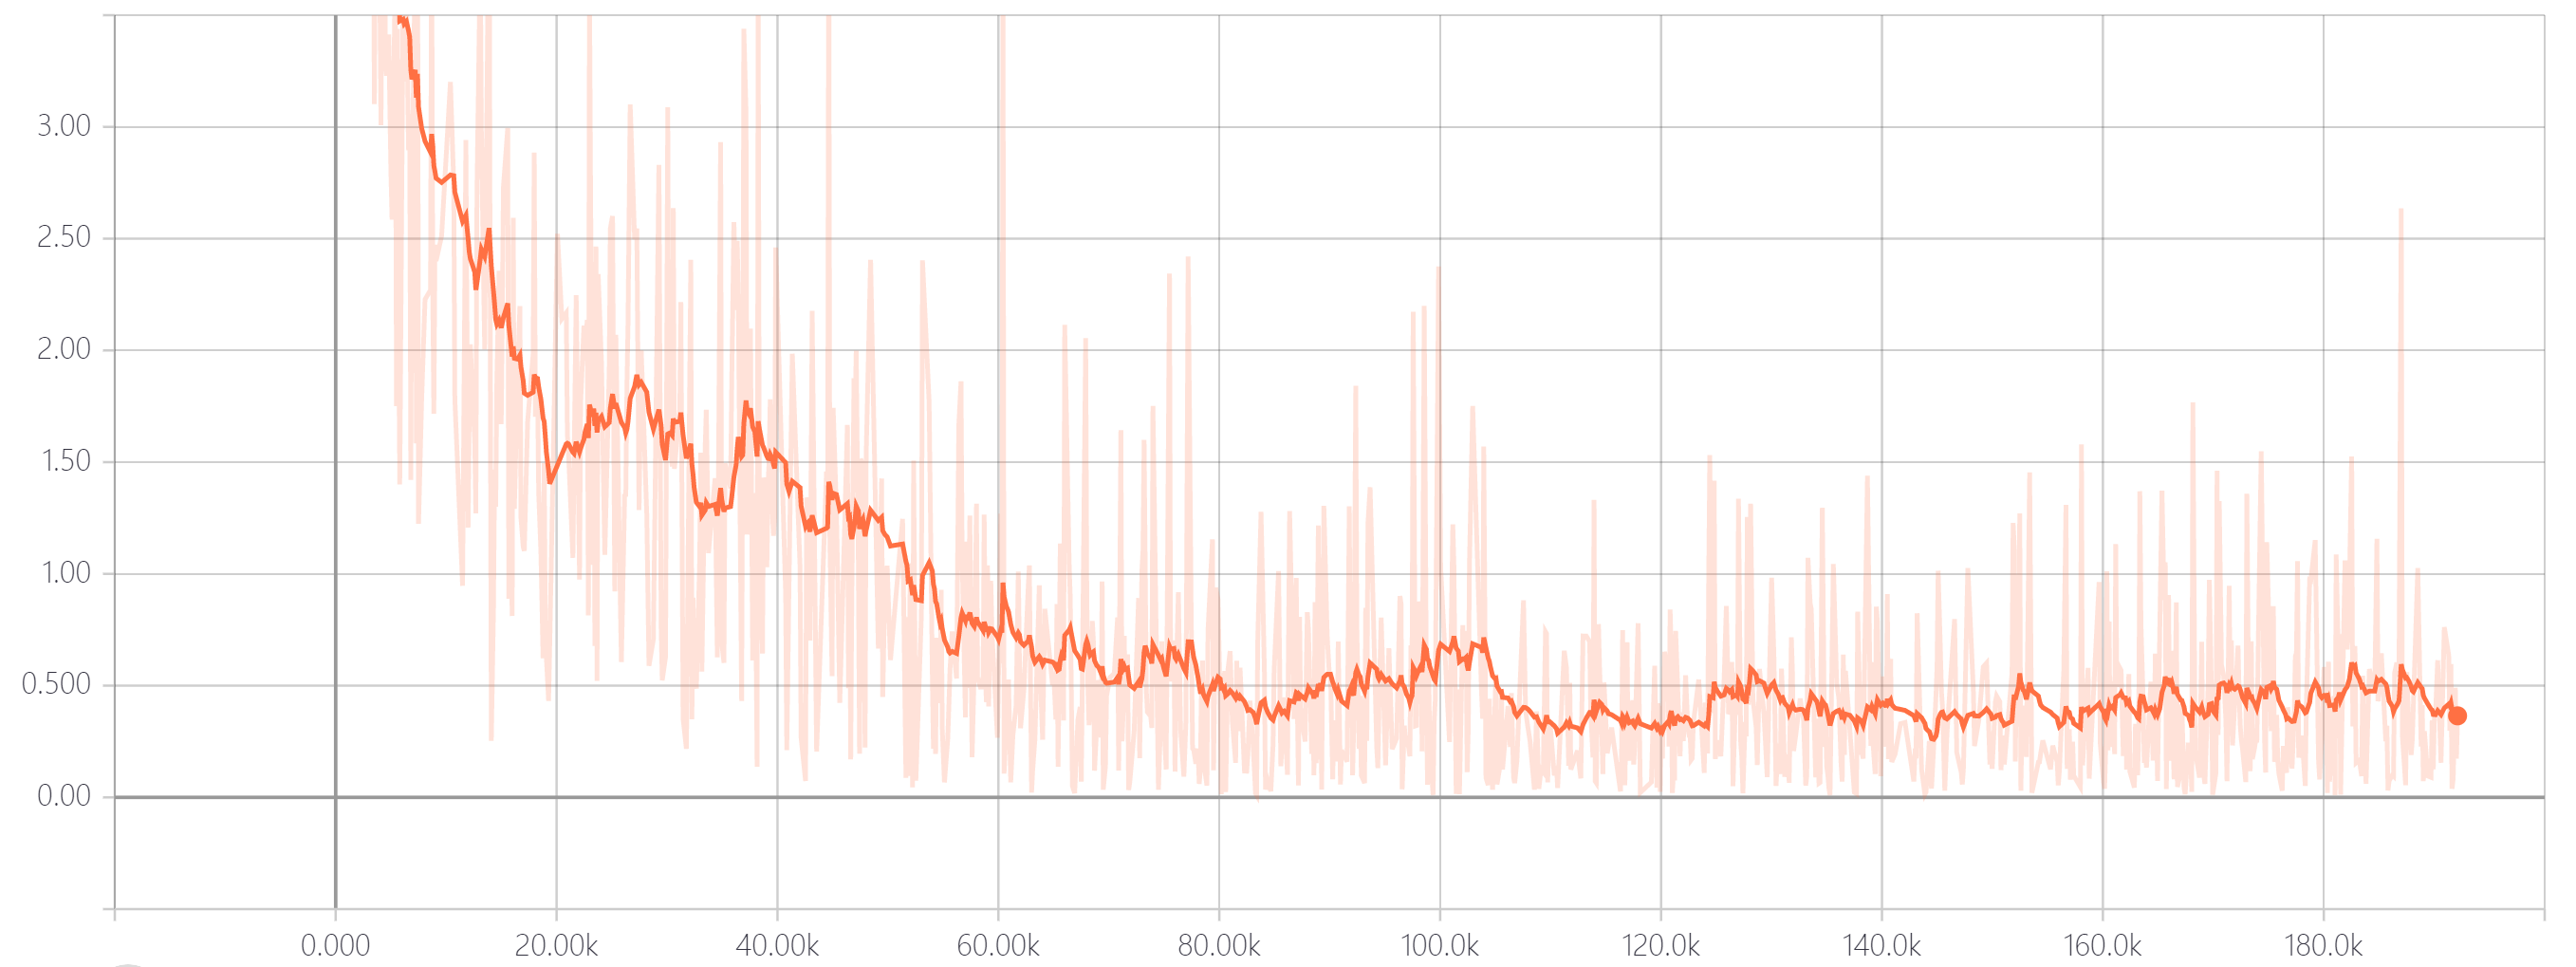
\includegraphics[width=0.75\textwidth]{resnet.png}
	\caption{Resnet训练曲线}
	\label{figure}
\end{figure*}

densenet在该数据集上获得了93.85\%的准确率,训练时的loss曲线如图5所示:

\begin{figure*}[htbp]
	\centering
	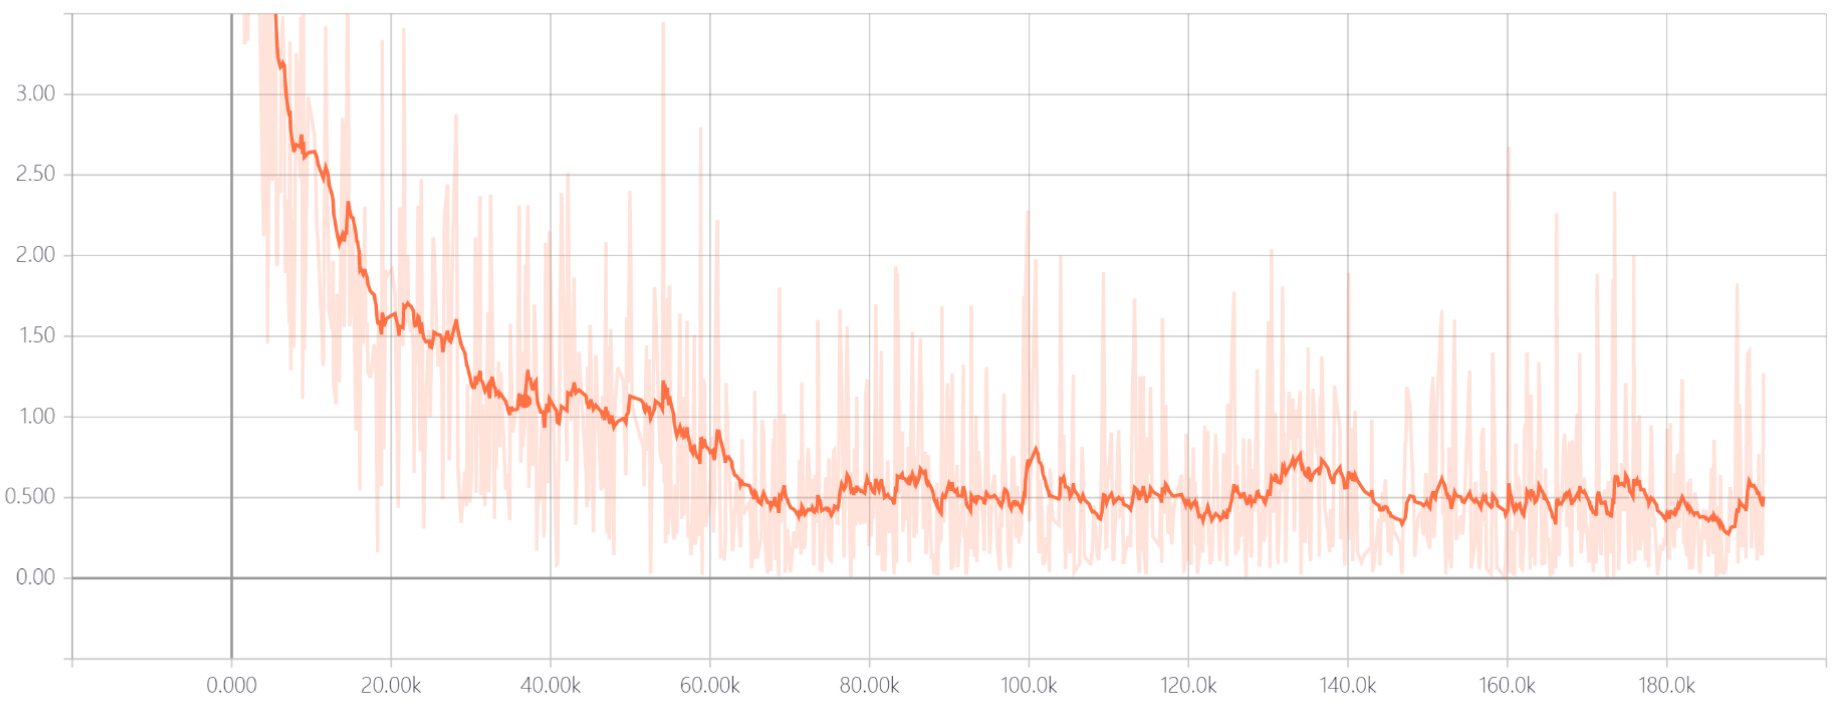
\includegraphics[width=0.75\textwidth]{densenet.png}
	\caption{Densenet训练曲线}
	\label{figure}
\end{figure*}
由上可见,三种模型对植物叶片图像分类的任务均有比较好的效果,而其中Densenet和Resnet训练的效果稍好,并且训练收敛的速度较快。

\subsection*{结果分析}

取densenet的数据进行结果分析,错误率较高的几个类别分别为:
\begin{center}
	\begin{tabular}{|c|c|}
		\hline 植物名称&错误率\\
		\hline prunus\_sargentii&27.4\%\\
		\hline prunus\_virginiana&23\%\\
		\hline quercus\_muehlenbergii&35\%\\
		\hline pinus\_virginiana&55\%\\
		\hline magnolia\_stellata&50\%\\
		\hline
	\end{tabular}
\end{center}
这些类别的叶片形状大致相似,比较难以区分,如图6所示:
	\begin{figure*}[htbp]
		\centering
		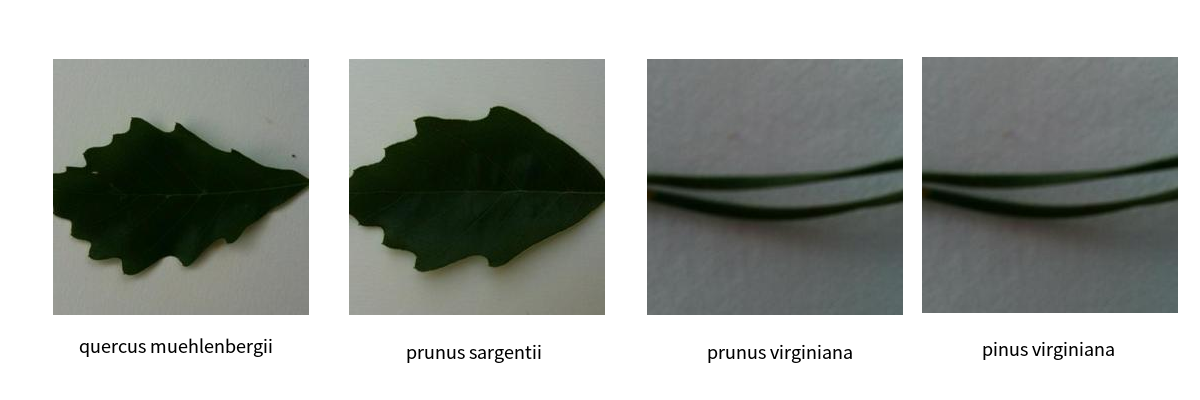
\includegraphics[width=0.75\textwidth]{img3.png}
		\caption{错误率较高的几个类别}
		\label{figure}
	\end{figure*}

观察图6,也有可能是数据集存在一些错误导致识别错误率较高。


\section*{结论}
我们在这篇论文中实现了三种深度学习模型,在已有的叶片数据集上进行了训练,显示出较好的结果,这些模型均可以用于植物图像识别的算法。但是这些算法依赖于大量的数据集,对植物叶片数据进行采集和人工分辨也需要耗费相当大的精力。另外,这些算法依赖于服务器上GPU的大规模运算,如果能将其适配于手持设备(如手机)上,则能够更加便于工作人员进行物种的调查采样。



\printbibliography[heading=none]
\end{document}